Estabelecidos os requisitos pretendidos para a
implementação, foram atualizados os modelos conceptuais
de forma a sustentar as novas funcionalidades pretendidas.
\newline

\subsection{Gerador de Primitivas}

\begin{center}
    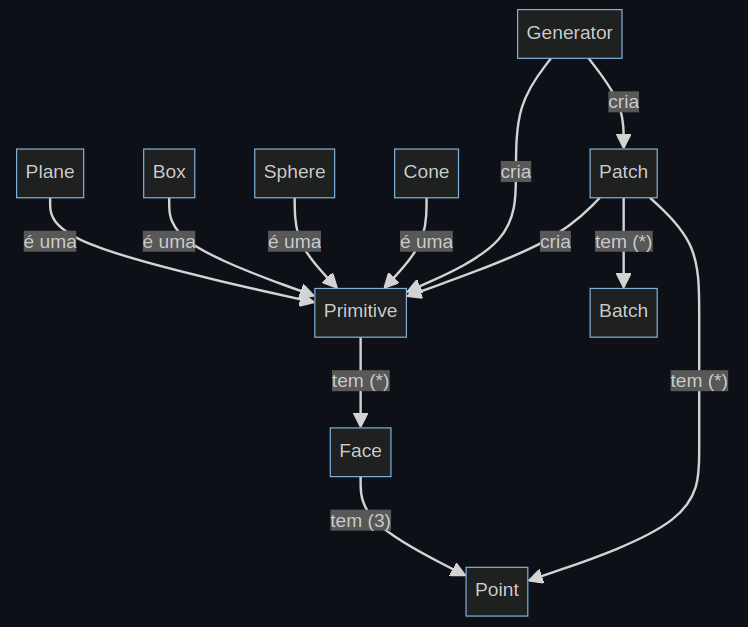
\includegraphics[width=0.8\textwidth]{imgs/concept1.png}
    \captionof{figure}{Modelo de Domínio do Gerador de Primitivas}
    \label{fig:domger}
\end{center}

\noindent
Reutilizando a abilidade já existente das primitivas de
gerarem ficheiros \textit{3d}, decidiu-se que será necessário
criar primeiro uma primitiva que represente um \textbf{patch}
e só em seguida escrevê-la em ficheiro.
\newline
\break
\noindent
Para tal, foi criada uma classe \textbf{Patch} que, recebendo
um ficheiro \textit{.patch}, gera uma primitiva. Esta fará uso,
ainda, de um conjunto de \textbf{Batches} que irão armazenar,
cada uma, um conjunto de índices de pontos (estes guardados
num conjunto de pontos também armazenado)
que representam uma superfície.
\newline
\break
\noindent
Cada \textbf{Batch} terá, então, de ser capaz de gerar a
superfície que representa, tal que, uma \textbf{Patch} possa
criar uma primitiva através do conjunto de superfícies
geradas.
\newline

\subsection{Motor gráfico}

\begin{center}
    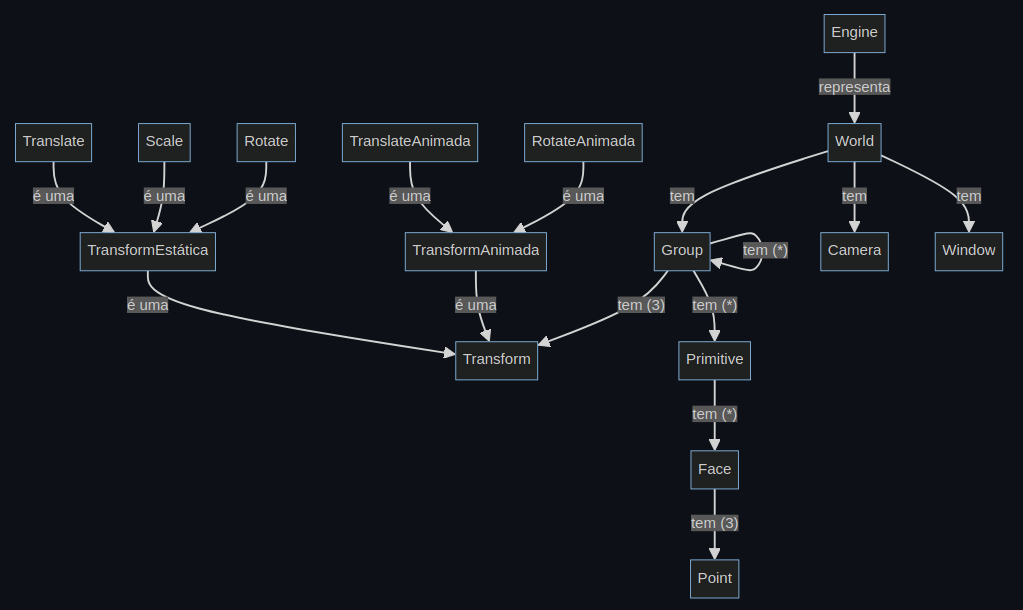
\includegraphics[width=0.8\textwidth]{imgs/concept2.png}
    \captionof{figure}{Modelo de Domínio do Motor Gráfico}
    \label{fig:domeng}
\end{center}

\noindent
Seguindo a hierarquia de transformações definida já na fase
anterior, foram adicionados novos elementos para a completar
de forma a possibilitar a animação.
\newline
\break
\noindent
Para tal, a hierarquia definida na fase anterior foi dada, agora,
como uma sub-hierarquia (TransformEstática) de um hierarquia
superior que contém todos os tipos de transformações.
\newline
\break
\noindent
Uma transformação passa, então, a definir as regras globais
de todas as transformações (tem de poder ser aplicadas) e as
transformações estática e animada definem as regras mais
especificas (tem de existir um eixo, no caso da transformação
estática, e tem de haver um intervalo de tempo, no caso
contrário).
\newline
\break
\noindent
As translações e rotações animadas definem, posteriormente,
as suas propriedades específicas, como o conjunto de pontos
que define a curva e o eixo de rotação, respetivamente.
\newline
\break
\noindent
Já os \textbf{VBO}s não apresentam necessidades de alteração
da arquitetura, tendo apenas atualizações relativas à
implementação.